\documentclass[../main.tex]{subfiles}

\begin{document}

\section{Planimetría}

\subsection{Curvas verticales}
Se comenzó dividiendo el camino en tres partes, separadas por su variación en el rumbo y con los datos proporcionados se procedió a calcular los demás rumbos y el ángulo interior faltante.

Para ello, a los 180º se le restó el ángulo y el rumbo dato en función de su orientación.

\begin{figure}[ht]
    \centering
    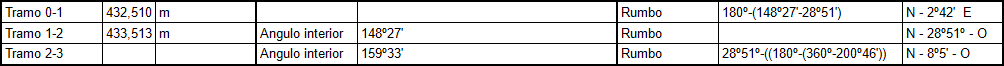
\includegraphics[width=\textwidth]{images/google_sheets/Screenshot_1.png}
    \caption{Cálculo de rumbos}
    \label{fig:rumbos}
\end{figure}


\subsubsection{Estudio General}
Se procedió con el cálculo de los ángulos de quiebre de alineamientos rectos, restándole a 180º los rumbos correspondientes. Luego se calculó el Radio Mínimo de la Curva Circular, según la tabla 5.1 obtenidos en 'Alineamiento Vial Planimétrico' de Cornero. \cite{cornero_planimetria}


Después, se seleccionó la mayor longitud espiral en función a la aceleración centrífuga (tabla 9.1), desarrollo del peralte (tabla 9.2) o apariencia del trazado (tabla 9.3). De las tablas 10.1 y 13.1 se determinó la longitud de la tangente extendida mínima y los sobreanchos en alineamientos curvos respectivamente. \cite{cornero_planimetria}

\begin{figure}[ht]
    \centering
    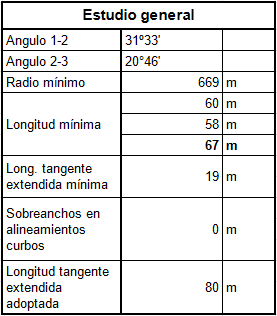
\includegraphics[width=0.4\textwidth]{images/google_sheets/Screenshot_2.png}
    \caption{Estudio general}
    \label{fig:estudio_general}
\end{figure}


\subsubsection{Curvas horizontales}
Con estos datos, se recurrió a las tablas de Barnett para el cálculo de la Longitud espiral en las cuales se realizó una interpolación para adoptar el correcto valor del ángulo de quiebre. Se procedió con la determinación de los parámetros $T_e$ y $E_e$, para lo cual se adoptó un radio óptimo determinado. Finalmente se procedió con la Tangente Extendida mediante semejanza de triángulos. Esto lo podemos ver en \cref{fig:curva1} y \cref{fig:curva2}.

\begin{figure}[ht]
\centering
\begin{subfigure}{.5\textwidth}
  \centering
  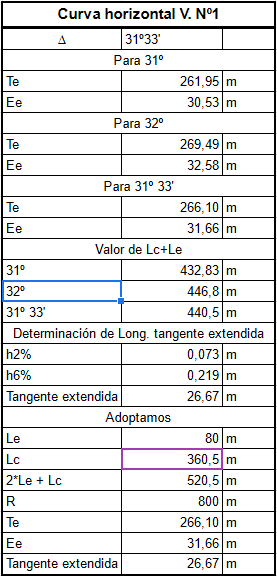
\includegraphics[width=0.85\linewidth]{images/google_sheets/Screenshot_3.png}
  \captionof{figure}{Curva horizontal Nº1}
  \label{fig:curva1}
\end{subfigure}%
\begin{subfigure}{.5\textwidth}
  \centering
  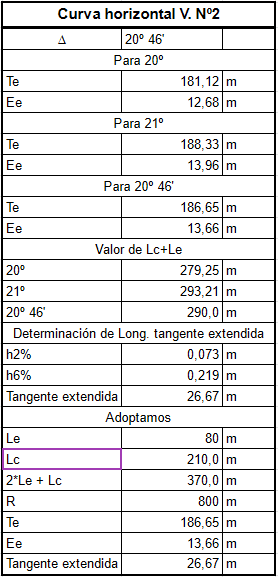
\includegraphics[width=0.85\linewidth]{images/google_sheets/Screenshot_4.png}
  \captionof{figure}{Curva horizontal Nº2}
  \label{fig:curva2}
\end{subfigure}
\caption{Parámetros de las curvas}
\end{figure}



\subsubsection{Determinación de progresivas}
Se realizó la determinación de las progresivas comenzando en el inicio de su tangente extendida y se procedió adicionando al valor inicial el porcentaje correspondiente de la longitud espiral y de la longitud de la curva en cuestión en función a la variación de las pendientes de la calzada 


\subsubsection{Cotas de borde}
Para el estudio de las Cotas de Borde se supuso una cota de la calzada determinada a la cual se le calculó la cota de borde normal en función a la pendiente de la calzada y del ancho de la misma, este proceso se repitió para todo el avance de la curva con las pendientes totales de 2\% y 4\%. El cálculo se encuentra en \cref{fig:cotas_bordes}.

\begin{figure}[ht]
    \centering
    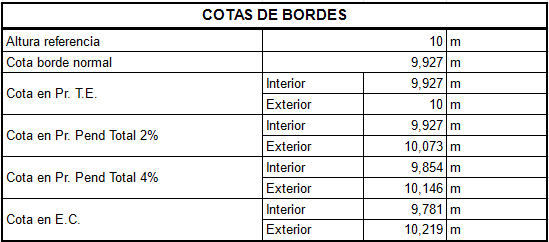
\includegraphics[width=0.575\textwidth]{images/google_sheets/Screenshot_5.png}
    \caption{Cotas de bordes}
    \label{fig:cotas_bordes}
\end{figure}

\end{document}